% Options for packages loaded elsewhere
\PassOptionsToPackage{unicode}{hyperref}
\PassOptionsToPackage{hyphens}{url}
\documentclass[
]{article}
\usepackage{xcolor}
\usepackage{amsmath,amssymb}
\setcounter{secnumdepth}{5}
\usepackage{iftex}
\ifPDFTeX
  \usepackage[T1]{fontenc}
  \usepackage[utf8]{inputenc}
  \usepackage{textcomp} % provide euro and other symbols
\else % if luatex or xetex
  \usepackage{unicode-math} % this also loads fontspec
  \defaultfontfeatures{Scale=MatchLowercase}
  \defaultfontfeatures[\rmfamily]{Ligatures=TeX,Scale=1}
\fi
% \usepackage{lmodern}
\ifPDFTeX\else
  % xetex/luatex font selection
\fi
% Use upquote if available, for straight quotes in verbatim environments
\IfFileExists{upquote.sty}{\usepackage{upquote}}{}
\IfFileExists{microtype.sty}{% use microtype if available
  \usepackage[]{microtype}
  \UseMicrotypeSet[protrusion]{basicmath} % disable protrusion for tt fonts
}{}
\makeatletter
\@ifundefined{KOMAClassName}{% if non-KOMA class
  \IfFileExists{parskip.sty}{%
    \usepackage{parskip}
  }{% else
    \setlength{\parindent}{0pt}
    \setlength{\parskip}{6pt plus 2pt minus 1pt}}
}{% if KOMA class
  \KOMAoptions{parskip=half}}
\makeatother
\usepackage{color}
\usepackage{fancyvrb}
\newcommand{\VerbBar}{|}
\newcommand{\VERB}{\Verb[commandchars=\\\{\}]}
\DefineVerbatimEnvironment{Highlighting}{Verbatim}{commandchars=\\\{\}}
% Add ',fontsize=\small' for more characters per line
\newenvironment{Shaded}{}{}
\newcommand{\AlertTok}[1]{\textcolor[rgb]{1.00,0.00,0.00}{\textbf{#1}}}
\newcommand{\AnnotationTok}[1]{\textcolor[rgb]{0.38,0.63,0.69}{\textbf{\textit{#1}}}}
\newcommand{\AttributeTok}[1]{\textcolor[rgb]{0.49,0.56,0.16}{#1}}
\newcommand{\BaseNTok}[1]{\textcolor[rgb]{0.25,0.63,0.44}{#1}}
\newcommand{\BuiltInTok}[1]{\textcolor[rgb]{0.00,0.50,0.00}{#1}}
\newcommand{\CharTok}[1]{\textcolor[rgb]{0.25,0.44,0.63}{#1}}
\newcommand{\CommentTok}[1]{\textcolor[rgb]{0.38,0.63,0.69}{\textit{#1}}}
\newcommand{\CommentVarTok}[1]{\textcolor[rgb]{0.38,0.63,0.69}{\textbf{\textit{#1}}}}
\newcommand{\ConstantTok}[1]{\textcolor[rgb]{0.53,0.00,0.00}{#1}}
\newcommand{\ControlFlowTok}[1]{\textcolor[rgb]{0.00,0.44,0.13}{\textbf{#1}}}
\newcommand{\DataTypeTok}[1]{\textcolor[rgb]{0.56,0.13,0.00}{#1}}
\newcommand{\DecValTok}[1]{\textcolor[rgb]{0.25,0.63,0.44}{#1}}
\newcommand{\DocumentationTok}[1]{\textcolor[rgb]{0.73,0.13,0.13}{\textit{#1}}}
\newcommand{\ErrorTok}[1]{\textcolor[rgb]{1.00,0.00,0.00}{\textbf{#1}}}
\newcommand{\ExtensionTok}[1]{#1}
\newcommand{\FloatTok}[1]{\textcolor[rgb]{0.25,0.63,0.44}{#1}}
\newcommand{\FunctionTok}[1]{\textcolor[rgb]{0.02,0.16,0.49}{#1}}
\newcommand{\ImportTok}[1]{\textcolor[rgb]{0.00,0.50,0.00}{\textbf{#1}}}
\newcommand{\InformationTok}[1]{\textcolor[rgb]{0.38,0.63,0.69}{\textbf{\textit{#1}}}}
\newcommand{\KeywordTok}[1]{\textcolor[rgb]{0.00,0.44,0.13}{\textbf{#1}}}
\newcommand{\NormalTok}[1]{#1}
\newcommand{\OperatorTok}[1]{\textcolor[rgb]{0.40,0.40,0.40}{#1}}
\newcommand{\OtherTok}[1]{\textcolor[rgb]{0.00,0.44,0.13}{#1}}
\newcommand{\PreprocessorTok}[1]{\textcolor[rgb]{0.74,0.48,0.00}{#1}}
\newcommand{\RegionMarkerTok}[1]{#1}
\newcommand{\SpecialCharTok}[1]{\textcolor[rgb]{0.25,0.44,0.63}{#1}}
\newcommand{\SpecialStringTok}[1]{\textcolor[rgb]{0.73,0.40,0.53}{#1}}
\newcommand{\StringTok}[1]{\textcolor[rgb]{0.25,0.44,0.63}{#1}}
\newcommand{\VariableTok}[1]{\textcolor[rgb]{0.10,0.09,0.49}{#1}}
\newcommand{\VerbatimStringTok}[1]{\textcolor[rgb]{0.25,0.44,0.63}{#1}}
\newcommand{\WarningTok}[1]{\textcolor[rgb]{0.38,0.63,0.69}{\textbf{\textit{#1}}}}
\usepackage{longtable,booktabs,array}
\newcounter{none} % for unnumbered tables
\usepackage{calc} % for calculating minipage widths
% Correct order of tables after \paragraph or \subparagraph
\usepackage{etoolbox}
\makeatletter
\patchcmd\longtable{\par}{\if@noskipsec\mbox{}\fi\par}{}{}
\makeatother
% Allow footnotes in longtable head/foot
\IfFileExists{footnotehyper.sty}{\usepackage{footnotehyper}}{\usepackage{footnote}}
\makesavenoteenv{longtable}
\usepackage{graphicx}
\makeatletter
\newsavebox\pandoc@box
\newcommand*\pandocbounded[1]{% scales image to fit in text height/width
  \sbox\pandoc@box{#1}%
  \Gscale@div\@tempa{\textheight}{\dimexpr\ht\pandoc@box+\dp\pandoc@box\relax}%
  \Gscale@div\@tempb{\linewidth}{\wd\pandoc@box}%
  \ifdim\@tempb\p@<\@tempa\p@\let\@tempa\@tempb\fi% select the smaller of both
  \ifdim\@tempa\p@<\p@\scalebox{\@tempa}{\usebox\pandoc@box}%
  \else\usebox{\pandoc@box}%
  \fi%
}
% Set default figure placement to htbp
\def\fps@figure{htbp}
\makeatother
\setlength{\emergencystretch}{3em} % prevent overfull lines
\providecommand{\tightlist}{%
  \setlength{\itemsep}{0pt}\setlength{\parskip}{0pt}}
\usepackage[]{natbib}
\bibliographystyle{plainnat}
\usepackage{bookmark}
\IfFileExists{xurl.sty}{\usepackage{xurl}}{} % add URL line breaks if available
\urlstyle{same}
\hypersetup{
  colorlinks=true,linkcolor=red,urlcolor=red,citecolor=red,anchorcolor=red,
  pdfcreator={LaTeX via pandoc}}

\author{}
\date{}

\title{Statistical Proximity of Irrational and Transcendental Constants to Bounded-Denominator Rationals\\\normalsize A reproducible Monte Carlo baseline}
\author{Research Template Author\\\footnotesize{Research Template Institute}\\\footnotesize{\texttt{author@research-template.org}}\\\footnotesize{\href{https://orcid.org/0000-0000-0000-0000}{ORCID: 0000-0000-0000-0000}}}
\date{\today}

% Core mathematics
\usepackage{amsmath}
\usepackage{amssymb}
\usepackage{amsfonts}
\usepackage{amsthm}

% Document layout
\usepackage{geometry}
\usepackage{float}
\usepackage{graphicx}

% Tables
\usepackage{booktabs}
\usepackage{longtable}
\usepackage{array}

% Code listings
\usepackage{listings}

% Typography and formatting
\usepackage{microtype}
\usepackage{xcolor}
\usepackage[binary-units]{siunitx}

% Cross-references and citations
\usepackage{hyperref}
\hypersetup{
    colorlinks=true,
    allcolors=red
}
\usepackage[capitalise,noabbrev]{cleveref}
\usepackage{natbib}

\begin{document}

\maketitle
\thispagestyle{empty}
\tableofcontents
\newpage


\section{Abstract}\label{abstract}

We quantify how close fixed mathematical constants lie to rationals
\(p/q\) with bounded denominator \(q \leq Q\), and contrast them against
Monte Carlo draws from reference ensembles on \([0,1)\) and from
fractional parts of square roots. The statistic is the elementary
minimum absolute error
\(\min_{p \in \mathbb{Z},\,1 \leq q \leq Q} |x - p/q|\), evaluated in
IEEE-754 double precision with deterministic seeds. Classical
Diophantine theory (Dirichlet, Hurwitz, Khinchin) explains why almost
every real admits arbitrarily sharp rational approximations as
\(Q \to \infty\); here we fix modest \(Q\) and compare empirical tail
placement of named constants (including a rational control) relative to
synthetic baselines. All computation lives in
\texttt{projects/special\_number\_proximity/src/} with a zero-mock test
suite; figures and tables are produced by
\texttt{scripts/proximity\_monte\_carlo.py}.

\textbf{Keywords:} Diophantine approximation, continued fractions, Monte
Carlo methods, reproducible computing

\newpage

\section{Introduction}\label{introduction}

Rational numbers are dense in the reals, yet the \emph{quality} of the
best approximation at a fixed denominator ceiling varies sharply across
individual \(x\). Number theory classifies extremes: algebraic
irrationals of degree two have bounded partial quotients in their
continued fraction expansion (hence are \emph{badly approximable}),
while almost every \(x\) satisfies Khinchin-type statistics for the
growth of those quotients \citep{khinchin1964continued}. Transcendental
numbers carry no algebraic constraint of that form, but individual
constants such as \(\pi) or \(e\) still exhibit structured rational
approximations arising from truncated series or independent
constructions.

This note does not prove new bounds. It implements a transparent,
test-backed pipeline that measures a single finite-\(Q\) statistic for
several standard constants and compares each value to the distribution
induced by simple random constructions. The goal is pedagogical and
methodological: link classical statements about limits as \(Q\to\infty\)
to observable finite-\(Q\) variation, and document the measurement chain
so others can change \(Q\), the reference law, or the constant registry
without touching infrastructure code.

\newpage

\section{Problem statement}\label{problem-statement}

Fix an integer \(Q \geq 1\). For a real \(x\), define \begin{equation}
\label{eq:delta}
\delta_Q(x) = \min_{p \in \mathbb{Z},\, 1 \leq q \leq Q} \left| x - \frac{p}{q} \right|.
\end{equation}

For analysis on the circle group \(\mathbb{R}/\mathbb{Z}\) one often
studies the fractional part \(\{x\}\) and the same functional with \(x\)
replaced by \(\{x\}\); the implementation exposes both the raw distance
on \(\mathbb{R}\) and the fractional variant used when comparing draws
supported on \([0,1)\).

\textbf{Research question (statistical).} Conditional on a chosen
reference law for \(X\) (uniform on \([0,1)\), or fractional parts
\(\{\sqrt{k}\}\) with random square-free \(k\)), where do deterministic
constants \(x^\star\) sit in the empirical distribution of
\(\delta_Q(X)\)? Equivalently: what empirical percentile does
\(\delta_Q(x^\star)\) attain relative to Monte Carlo samples at the same
\(Q\)?

\textbf{Rational control.} Any \(x \in \mathbb{Q}\) yields
\(\delta_Q(x)=0\) once \(Q\) exceeds the reduced denominator of \(x\),
providing a structural sanity check on the implementation.

\newpage

\section{Measure-theoretic context
(qualitative)}\label{measure-theoretic-context-qualitative}

\subsection{Almost every number is well
approximable}\label{almost-every-number-is-well-approximable}

Dirichlet's theorem guarantees that for every irrational \(x\) and every
\(Q>1\) there exist integers \(p,q\) with \(1 \leq q \leq Q\) and
\(|qx - p| < 1/Q\), hence \(|x - p/q| < 1/qQ \leq 1/Q\). Thus
\(\delta_Q(x) \leq 1/Q\) always for irrational \(x\); the interesting
variation is sub-leading in \(Q\).

\subsection{Badly approximable
numbers}\label{badly-approximable-numbers}

An irrational \(x\) is \emph{badly approximable} if there exists \(c>0\)
such that \(|x - p/q| > c/q^2\) for all rationals \(p/q\). Equivalently,
the partial quotients in the continued fraction expansion of \(x\) are
bounded. Quadratic irrationals, including the golden ratio \(\varphi\),
belong to this class \citep{cassels1957}. At fixed \(Q\), such numbers
tend to sit in less extreme left tails of \(\delta_Q\) than typical
draws from uniform \([0,1)\)---they resist \emph{especially} close
low-denominator hits.

\subsection{\texorpdfstring{What transcendence does not encode at fixed
\(Q\)}{What transcendence does not encode at fixed Q}}\label{what-transcendence-does-not-encode-at-fixed-q}

Being transcendental rules out exact satisfaction of a nontrivial
integer polynomial, but it does not by itself determine \(\delta_Q(x)\)
at moderate \(Q\) in double precision. Empirical comparison against
random baselines therefore remains informative for exposition even when
classical transcendentality proofs are orthogonal to the statistic
\eqref{eq:delta}.

\newpage

\section{Continued fractions as an explanatory
tool}\label{continued-fractions-as-an-explanatory-tool}

The source module \texttt{continued\_fractions.py} exposes partial
quotients \([a_0; a_1, a_2, \ldots]\) for positive floats and exact
Euclidean continued fractions for positive rationals \(p/q\).
Convergents \(p_k/q_k\) satisfy the recurrence \begin{align}
p_k &= a_k p_{k-1} + p_{k-2}, \\
q_k &= a_k q_{k-1} + q_{k-2},
\end{align} initialized by \((p_{-1},q_{-1})=(1,0)\),
\((p_0,q_0)=(a_0,1)\) in the standard indexing shift used in code.

For \(\varphi = (1+\sqrt{5})/2\), one expects \(a_i=1\) for all
\(i \geq 1\) under exact arithmetic; floating expansion truncates once
rounding breaks the fixed point of the Gauss map.

The statistic \(\delta_Q(x)\) in \eqref{eq:delta} is computed
independently by scanning denominators \(1 \leq q \leq Q\) and three
candidate numerators around \(xq\); this \(O(Q)\) method is exact for
double-\(x\) at the stated grid and is simpler to test than full
semiconvergent enumeration while remaining adequate for the Monte Carlo
scales used here.

\newpage

\section{Monte Carlo design}\label{monte-carlo-design}

\subsection{Reference samples}\label{reference-samples}

The analysis script \texttt{proximity\_monte\_carlo.py} draws:

\begin{enumerate}
\def\labelenumi{\arabic{enumi}.}
\tightlist
\item
  \textbf{Uniform baseline:} \(U_1,\ldots,U_n \sim \mathrm{Unif}(0,1)\).
\item
  \textbf{Quadratic fractional baseline:} values \(\{\sqrt{k}\}\) for
  \(k\) sampled with replacement from a fixed list of small square-free
  integers.
\item
  \textbf{Optional Beta baseline:} if
  \texttt{experiment.n\_beta\ \textgreater{}\ 0}, additional draws
  \(B_i \sim \mathrm{Beta}(a,b)\) on \((0,1)\) (parameters
  \texttt{beta\_a}, \texttt{beta\_b}, default \(1/2\), \(1/2\)) are
  included to stress U-shaped or boundary-heavy laws.
\end{enumerate}

All streams share one NumPy \texttt{Generator} seeded from
\texttt{manuscript/config.yaml} (\texttt{experiment.rng\_seed}).
Distances \(\delta_Q\) are concatenated into a pooled reference; JSON
output includes \texttt{reference\_summary} (count, mean, selected
quantiles) for quick tables.

\subsection{Constants}\label{constants}

\texttt{constants.py} registers \(\pi), \(e\), \(\sqrt{2}\),
\(\sqrt{3}\), \(\varphi\), \(\ln 2\), and \(1/6\) (rational control).
Labels such as \texttt{transcendental} versus
\texttt{irrational\_algebraic} are documentary; proofs are not
recomputed in software.

\subsection{Outputs}\label{outputs}

Structured JSON and CSV land in \texttt{output/data/}; a log-scale
histogram of the uniform baseline with vertical markers for selected
constants is written to \texttt{../figures/proximity\_histogram.png}.

A second script, \texttt{02\_lattice\_crosscheck.py}, writes
\texttt{output/data/lattice\_crosscheck.json} comparing brute-force
\(\delta_Q\) to the scaled-lattice formulation and recording Dirichlet
residual checks.

Parameters \texttt{q\_max}, \texttt{n\_uniform}, \texttt{n\_quadratic},
\texttt{n\_beta}, \texttt{beta\_a}, and \texttt{beta\_b} are
YAML-configurable to respect the template's reproducibility contract
without code edits.

\newpage

\section{Scaled lattice and Dirichlet
residual}\label{scaled-lattice-and-dirichlet-residual}

\subsection{Identity}\label{identity}

For \(q \in \mathbb{N}\) and \(x \in \mathbb{R}\), write
\(\|y\| := \mathrm{dist}(y,\mathbb{Z})\). Choosing
\(p = \mathrm{round}(qx)\) minimises \(|qx - p|\), hence

\[
\left|x - \frac{p}{q}\right| = \frac{\|qx\|}{q}.
\]

Therefore the bounded-denominator functional from
\texttt{02\_problem\_statement.md} satisfies

\[
\delta_Q(x) = \min_{1 \leq q \leq Q} \frac{\|qx\|}{q}.
\]

The implementation
\texttt{min\_rational\_distance\_via\_scaled\_lattice} in
\texttt{diophantine\_bounds.py} evaluates this form; it agrees with the
brute-force search in \texttt{rational\_distance.py} for every tested
pair \((x,Q)\) (see \texttt{output/data/lattice\_crosscheck.json} from
\texttt{02\_lattice\_crosscheck.py}).

\subsection{Pigeonhole bound on the integer
residual}\label{pigeonhole-bound-on-the-integer-residual}

The classical box argument shows that for each \(Q \geq 1\) there exists
\(q \in \{1,\ldots,Q\}\) with \(\|qx\| \leq 1/(Q+1)\)
\citep{cassels1957}. This controls the \textbf{numerator} \(\|qx\|\)
only; dividing by \(q\) to compare with \(\delta_Q(x)\) requires the
separate optimisation above.

\subsection{Relation to continued
fractions}\label{relation-to-continued-fractions}

Continued-fraction convergents supply excellent rational approximations
but need not attain \(\delta_Q(x)\) for a fixed \(Q\) without
semiconvergents; \texttt{cf\_distance.py} documents the convergent-only
lower envelope used for quick certificates.

\newpage

\section{Results}\label{results}

All numbers below come from \texttt{output/data/proximity\_summary.json}
after running \texttt{scripts/proximity\_monte\_carlo.py} with
\texttt{q\_max=120}, \texttt{n\_uniform=4000},
\texttt{n\_quadratic=2000}, \texttt{n\_beta=1000} (Jeffreys prior on
\((0,1)\)), seed \texttt{20260322} (see
\texttt{manuscript/config.yaml}). The same JSON carries
\texttt{reference\_summary} for the pooled sample. Independent checks of
the \(\delta_Q\) implementation appear in
\texttt{output/data/lattice\_crosscheck.json} from
\texttt{02\_lattice\_crosscheck.py}.

\subsection{\texorpdfstring{Empirical percentiles of
\(\delta_{120}(x^\star)\)}{Empirical percentiles of \textbackslash delta\_\{120\}(x\^{}\textbackslash star)}}\label{empirical-percentiles-of-delta_120xstar}

{\def\LTcaptype{none} % do not increment counter
\begin{longtable}[]{@{}
  >{\raggedright\arraybackslash}p{(\linewidth - 4\tabcolsep) * \real{0.1389}}
  >{\raggedright\arraybackslash}p{(\linewidth - 4\tabcolsep) * \real{0.3472}}
  >{\raggedright\arraybackslash}p{(\linewidth - 4\tabcolsep) * \real{0.5139}}@{}}
\toprule\noalign{}
\begin{minipage}[b]{\linewidth}\raggedright
Constant
\end{minipage} & \begin{minipage}[b]{\linewidth}\raggedright
\(\delta_{120}(x^\star)\)
\end{minipage} & \begin{minipage}[b]{\linewidth}\raggedright
empirical rank in pooled reference
\end{minipage} \\
\midrule\noalign{}
\endhead
\bottomrule\noalign{}
\endlastfoot
\texttt{one\_sixth} (rational) & \(0\) & \(0\) \\
\texttt{pi} & \(2.67\times 10^{-7}\) & \(0.00171\) \\
\texttt{e} & \(2.80\times 10^{-5}\) & \(0.192\) \\
\texttt{ln2} & \(3.46\times 10^{-5}\) & \(0.279\) \\
\texttt{golden\_ratio} & \(5.65\times 10^{-5}\) & \(0.498\) \\
\texttt{sqrt2} & \(7.21\times 10^{-5}\) & \(0.574\) \\
\texttt{sqrt3} & \(9.20\times 10^{-5}\) & \(0.718\) \\
\end{longtable}
}

The rational control hits zero distance as soon as \(Q\) is a multiple
of the true denominator, confirming the end-to-end path from
\texttt{rational\_distance.py} through aggregation. \(\pi) occupies an
extreme left tail at this \(Q\)---consistent with the existence of
exceptionally accurate low-height rationals (e.g., \(355/113\)) that
remain admissible when \(Q=120\).

\subsection{Histogram}\label{histogram}

Figure \ref{fig:proximity_hist} shows the base-10 logarithm of
\(\delta_{120}(U)\) for uniform draws, with vertical markers for
\(\pi), \(\sqrt{2}\), \(\varphi\), and \(\ln 2\).

\begin{figure}
\centering
\pandocbounded{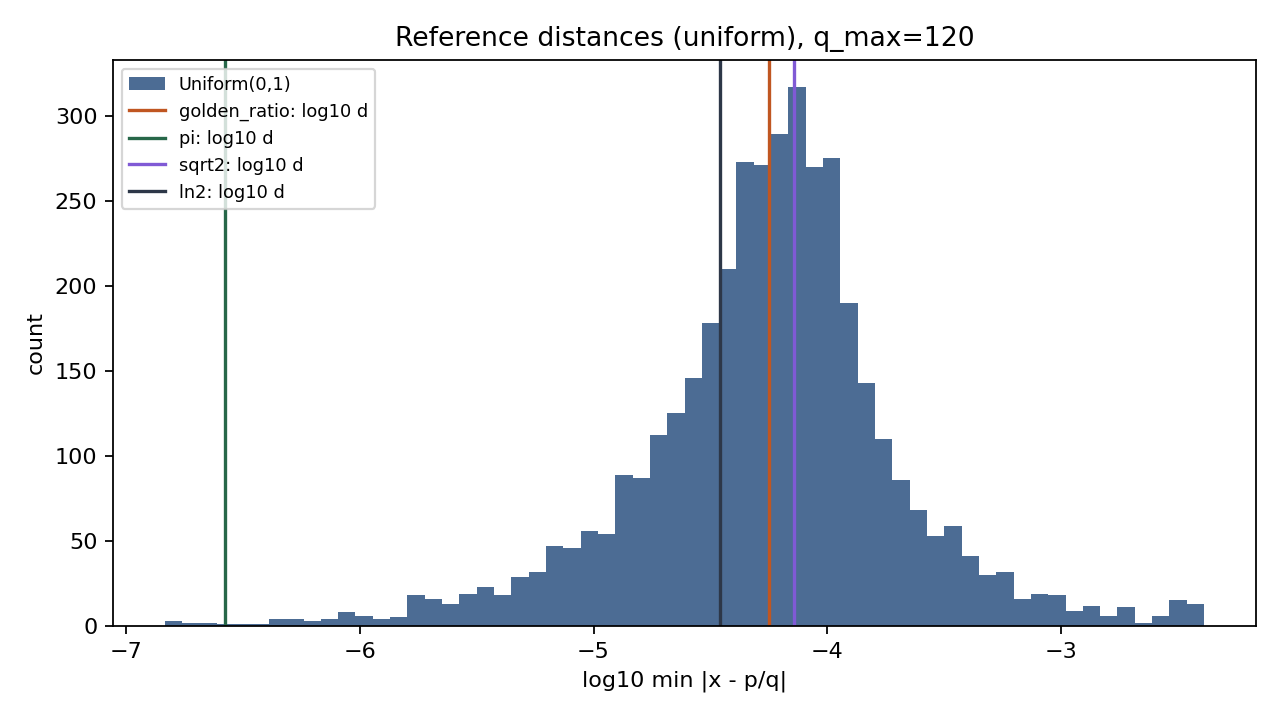
\includegraphics[keepaspectratio,alt={Empirical distribution of \textbackslash log\_\{10\} \textbackslash delta\_\{120\} for uniform references with marker lines for selected constants.}]{../figures/proximity_histogram.png}}
\caption{Empirical distribution of \(\log_{10} \delta_{120}\) for
uniform references with marker lines for selected
constants.}\label{fig:proximity_hist}
\end{figure}

The pooled reference (not plotted) adds quadratic-mod-\(1\) samples;
table ranks use that pooled empirical CDF.

\newpage

\section{Conclusion}\label{conclusion}

Finite-\(Q\) rational proximity is a coarse lens: it rewards numbers
that admit unusually accurate low-height approximations, not
``randomness'' in a probabilistic sense. At \(Q=120\), \(\pi) is a
visible outlier relative to uniform draws, while the golden ratio sits
near the median of the pooled reference---consistent with its badly
approximable, bounded-quotient profile at the level of heuristics. The
pipeline is modular (\texttt{continued\_fractions},
\texttt{rational\_distance}, \texttt{sampling},
\texttt{statistics\_compare}), fully tested without mocks, and
parameterized from YAML so \(Q\) and baselines can be altered for
coursework or further experiments.

\newpage

\section{Reproducibility}\label{reproducibility}

\subsection{Software}\label{software}

\begin{itemize}
\tightlist
\item
  Python \(\geq 3.10\), NumPy, Matplotlib, PyYAML (declared in
  \texttt{projects/special\_number\_proximity/pyproject.toml}; root
  \texttt{uv\ sync} supplies the environment).
\item
  Tests:
  \texttt{uv\ run\ pytest\ projects/special\_number\_proximity/tests/\ -\/-cov=projects/special\_number\_proximity/src\ -\/-cov-fail-under=90}.
\end{itemize}

\subsection{Regenerating artifacts}\label{regenerating-artifacts}

\begin{Shaded}
\begin{Highlighting}[]
\ExtensionTok{uv}\NormalTok{ run python projects/special\_number\_proximity/scripts/proximity\_monte\_carlo.py}
\end{Highlighting}
\end{Shaded}

Edits to \texttt{manuscript/config.yaml} under \texttt{experiment:}
change seeds, sample sizes, and \(Q\) without touching Python sources.

\subsection{Data paths}\label{data-paths}

{\def\LTcaptype{none} % do not increment counter
\begin{longtable}[]{@{}
  >{\raggedright\arraybackslash}p{(\linewidth - 2\tabcolsep) * \real{0.6250}}
  >{\raggedright\arraybackslash}p{(\linewidth - 2\tabcolsep) * \real{0.3750}}@{}}
\toprule\noalign{}
\begin{minipage}[b]{\linewidth}\raggedright
Artifact
\end{minipage} & \begin{minipage}[b]{\linewidth}\raggedright
Path
\end{minipage} \\
\midrule\noalign{}
\endhead
\bottomrule\noalign{}
\endlastfoot
Summary JSON &
\texttt{projects/special\_number\_proximity/output/data/proximity\_summary.json} \\
Table CSV &
\texttt{projects/special\_number\_proximity/output/data/proximity\_constants.csv} \\
Figure &
\texttt{projects/special\_number\_proximity/../figures/proximity\_histogram.png} \\
\end{longtable}
}

\newpage

\section{Manuscript syntax}\label{manuscript-syntax}

\begin{itemize}
\tightlist
\item
  Citations: \texttt{{[}@khinchin1964continued{]}}; keys must exist in
  \texttt{references.bib}.
\item
  Equations: use \texttt{\textbackslash{}begin\{equation\}} /
  \texttt{\textbackslash{}label\{eq:...\}}; reference with
  \texttt{\textbackslash{}ref\{eq:...\}}.
\item
  Figures:
  \texttt{!{[}caption{]}(../figures/proximity\_histogram.png)\{\#fig:label\}}
  then \texttt{\textbackslash{}ref\{fig:label\}} in prose.
\end{itemize}

See \texttt{infrastructure/rendering} for Pandoc and crossref details.



\bibliography{references}
\end{document}
